%%%%%%%%%%%%%%%%%%%%%%%%%%%%%%%%%%%%%%%%%%%%%%%%%%%%%%%%%%%%%%%%%%%%%%%%%%%%%%%%%%%%%%%%%%%%%%%%%%%%%%%%%%%%%%%%%%%%%%%%%%%% 
% Latex Vorlage f�r Vortr�ge ES
%
% Autor: R. Marchthaler
%
%%%%%%%%%%%%%%%%%%%%%%%%%%%%%%%%%%%%%%%%%%%%%%%%%%%%%%%%%%%%%%%%%%%%%%%%%%%%%%%%%%%%%%%%%%%%%%%%%%%%%%%%%%%%%%%%%%%%%%%%%%%%%

\documentclass[a4paper,fleqn,twocolumn]{article} 

% Zusatzpakete laden:
\usepackage{enumerate,mathptmx,ngerman,graphicx,hhline,array,float,amssymb,amsmath,enumerate,ulem,fancyhdr,caption,url}
\usepackage{subfigure,amsmath,units,savefnmark,tabularx,float,booktabs}
%\usepackage[ngerman]{babel}
\usepackage[T1]{fontenc} 

% Inhaltsverzeichnis anpassen
\usepackage{titletoc} 
\dottedcontents{part}[2mm]{\large\fillast}{1mm}{0.5pc}


\usepackage[ngerman]{varioref}
%\usepackage{pstricks}		
\usepackage[latin1]{inputenc}
\usepackage{listings}														% Einbinden von Codelistings
\usepackage{xcolor,color}												% Einbinden von Farben
\usepackage[colorlinks=true, breaklinks=true, pdfborder={0 0 0}, pdftex, urlcolor=blue, citecolor=blue, linkcolor=blue]{hyperref} 


% description Anpassung, damit es sch�ner aussieht.
\usepackage{eqlist}
\let\description=\eqlist
\let\enddescription=\endeqlist
\let\eqlistlabel\descriptionlabel


% Layout:
\setlength{\topmargin}{-20mm}										% Abstand Seitenkopf vom Rand (0mm entspricht einem Abstand von 25.4mm)
\setlength{\headheight}{15mm}										% H�he Seitenkopfs
\setlength{\headsep}{15mm}											% Abstand Seitenkopf vom Seitenrumpf
\setlength{\textheight}{240mm}									% H�he Seitenrumpf 
\setlength{\footskip}{10mm}											% Abstand unteres Ende Seitenfuss zum unteren Ende Seitenrumpf 
\setlength{\oddsidemargin}{-9.4mm}							% Abstand ungerade Seitenzahlen vom Seitenrand 
                                                % (0mm entspricht einem Abstand vom Rand von 25.4mm)
\setlength{\evensidemargin}{-9.4mm} 						% Abstand ungerade Seitenzahlen vom Seitenrand
                                                % (0mm entspricht einem Abstand vom Rand von 25.4mm)
\setlength{\textwidth}{184mm} 									% Breite Seitenrumpf 

% Erstzeileneinzug:
\setlength{\parindent}{0.0em} 

% Abstand zwischen zwei Abs�tzen:
\setlength{\parskip}{6pt plus2pt minus2pt} 			% Setzt den vertikalen Abstand zwischen Abs�tzen auf 6 pt
																								% Das Plus und Minus f�gt Glue ein, d. h. TeX darf den Abstand um 4 Punkte
																								% vergr��ern oder verkleinern, um ein gutes Layout zu erzeugen 
																								% (z. B. b�ndiger Abschluss der Seite)
																		
% Kopf- unf Fu�zeile:
\pagestyle{fancy}																% Seitenlayout auf eigene Kopf- und Kopfzeilen �ndern
\fancyhf{}													  					% Kopf- und Fu�zeile l�schen
\renewcommand{\headrulewidth}{0.1pt}						% Srichst�rke der Line unterhalb der Kopfzeile
\renewcommand{\footrulewidth}{0.1pt}						% Srichst�rke der Line oberhalb der Fu�zeile
\rhead{
\includegraphics[width=4cm]{HE_Logo.pdf}}% Logo in der Kofzeile rechts platzieren
\cfoot{\footnotesize{- \thepage -}}             % Seitenzahl in der Fu�zeile mittig platzieren

% neu Defintion von Kopf- und Fu0zeilen einer leeren Seite (Titelseite, Inhaltsverzeichnis, etc.)
\fancypagestyle{plain}{
   \fancyhf{}
   \fancyhead[C]{} 											% alles ausblenden
   \renewcommand{\headrulewidth}{0.0pt} % Line unterhalb der Kopfzeile ausblenden
   \renewcommand{\footrulewidth}{0.1pt}	% Srichst�rke der Line oberhalb der Fu�zeile
   \cfoot{\footnotesize{- \thepage -}}             % Seitenzahl in der Fu�zeile mittig platzieren
}	

																				
\sloppy

%-----------------------------------------------------------------------------------------------------------------------
\begin{document}

\title{\Huge{Vortragsreihe\\[5mm] Embedded Systems Design\\[5mm]}}
\author{\Large{TIB6}}
\date{Sommersemester 2019}
\maketitle

\clearpage
\tableofcontents

\cleardoublepage
%---------------------------------------------------------------------------------------------------------------------------
% Kopf des Vortrags
%---------------------------------------------------------------------------------------------------------------------------

\part{Sensordatenfusion}
\begin{center}
Janfabian Fabriczek, \\ Geschwister-Scholl-Stra�e 15, 73732 Esslingen,\\ E-Mail: janfabian.fabriczek@stud.hs-esslingen.de \\[1cm] 18. April 2019 \\[1cm]
\end{center}


%---------------------------------------------------------------------------------------------------------------------------
% Textteil
%---------------------------------------------------------------------------------------------------------------------------
\section*{Einleitung und Motivation}

Das autonome Fahren hat f�r die Automobilbranche einen hohen Stellenwert. Ein Computer steuert das Automobil ohne menschlichen Einfluss. Damit der Computer im Automobil genau wei�, wie, wann und wo es fahren kann und muss, muss es die Umgebung wahrnehmen k�nnen.

Um die Umgebung wahrnehmen zu k�nnen, werden Sensoren am Automobil verwendet. In der Au�enwelt gibt es viele verschiedene Wetterbedingungen, die die Sensoren so stark beeinflussen k�nnen, dass sie ihren Zweck nicht mehr erf�llen k�nnen. Der Einsatz mehrerer Sensoren mit unterschiedlichen Wahrnehmungsverfahren hilft dabei, die Blindheit des Automobils zu vermeiden und somit auch die Sicherheit neben der Funktionsf�higkeit zu gew�hrleisten.

Der Einsatz von mehreren Sensoren erfordert allerdings, dass die Messdaten zusammengefasst werden und unter Verwendung der zusammengefassten Messdaten ein komplettes Abbild der Umgebung erstellt wird. Unter dem Begriff \textit{Sensordatenfusion} wird das Zusammenf�hren der Sensordaten verstanden.


%%%%%%%%%%%%%%%%%%%%%%%%%%%%%%%%%%%%%%%%%%%%%%%%%%%%%%%%%%%%%%%%%%%%%%%%%%%%%%%

\newpage
\section*{Aufbau}

\subsection*{Allgemein}

Die einzelnen Sensoren sind �ber eine Verbindung mit dem Verarbeitungssystem verbunden \cite{Ref_WikiSDF}. Das Verarbeitungssystem fusioniert die Daten der einzelnen Sensoren \cite{Ref_WikiSDF}. Die Anwendungen greifen auf das Verarbeitungssystem zu, um die fusionierten Daten verwenden zu k�nnen \cite{Ref_WikiSDF}. Die zugreifende Anwendung kann basierend auf den vorhandenen Daten Entscheidungen treffen. In Abbildung \ref{Abb_AufbauSensordatenfusion} ist der Aufbau eines Systems zur Sensordatenfusion dargestellt.

%+++++++++++++++++++++++++++++++++++++++++++++++++++++++++++++
\begin{figure}[ht]
 \centerline{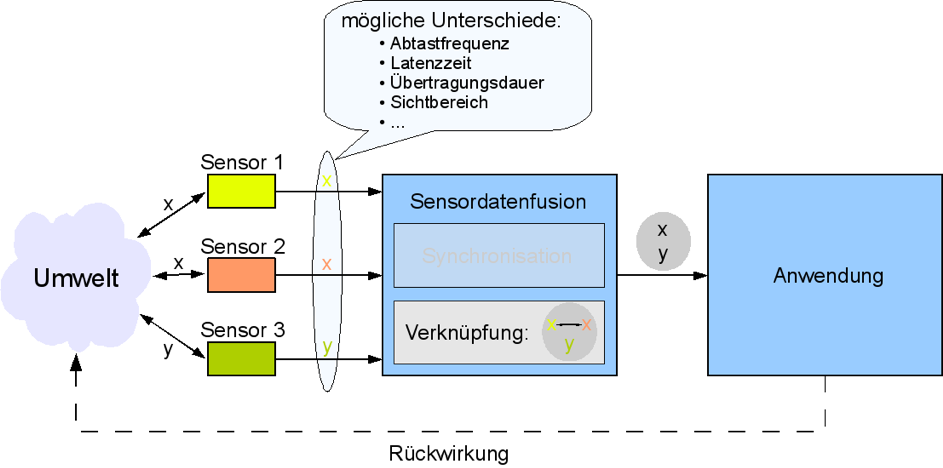
\includegraphics[width=0.41\textwidth]{Name_JFBR/aufbau_allgemein.png}}
 \caption {Aufbau eines Systems zur Sensordatenfusion \cite{Ref_WikiSDF}}
 \label{Abb_AufbauSensordatenfusion} 
\end{figure}
%+++++++++++++++++++++++++++++++++++++++++++++++++++++++++++++

Die Sensoren werden f�r die Sensordatenfusion nach einer bestimmten Strategie gew�hlt und angeordnet. Die einzelnen Strategien werden im Folgenden behandelt.

\subsection*{Sensoranordnung}

Die Sensoren werden in einem oder mehreren Sensornetzwerken angeordnet \cite{Ref_StuekerHomogeneSDF}.

Unter einem Sensornetzwerk wird der Verbund mehrerer gleicher oder auch unterschiedlicher Sensoren in einem Netzwerk verstanden.

Die Sensornetzwerke werden zwischen zwei Typen unterschieden \cite{Ref_StuekerHomogeneSDF}. Der eine Typ ist das homogene Sensornetzwerk und der andere Typ ist das heterogene Sensornetzwerk \cite{Ref_StuekerHomogeneSDF}.

In einem homogenen Sensornetzwerk verwenden alle Sensoren dasselbe physikalische Prinzip zum Messen. Die Sensoren in einem solchen Netzwerk unterliegen daher alle den gleichen Einschr�nkungen \cite{Ref_StuekerHomogeneSDF}.

In einem heterogenen Sensornetzwerk verwenden die Sensoren unterschiedliche physikalische Prinzipien zum Messen \cite{Ref_StuekerHomogeneSDF}. Die Sensoren in einem heterogenen Sensornetzwerk kompensieren die Einschr�nkungen einzelner Sensoren \cite{Ref_StuekerHomogeneSDF}.


%%%%%%%%%%%%%%%%%%%%%%%%%%%%%%%%%%%%%%%%%%%%%%%%%%%%%%%%%%%%%%%%%%%%%%%%%%%%%%%

\newpage


\section*{Funktionsweise}

\subsection*{Allgemein}

Die Fusion wird von einem Verarbeitungssystem unter der Verwendung von Algorithmen und mathematischen Verfahren durchgef�hrt. Bei der Fusion werden die Daten der einzelnen Sensoren synchronisiert, mehrere Eigenschaften zu neuen Eigenschaften zusammengef�gt und einzelne Erfassungsbereiche zu einem gr��eren Erfassungsbereich zusammengef�gt.

\subsection*{Fusionstypen}

Bei der Fusion wird zwischen Fusionstypen unterschieden. Der gew�hlte Fusionstyp hat Auswirkung auf die Sensorenauswahl und wof�r die Messdaten der Sensoren bei der Fusion verwendet werden. Im Folgenden werden die einzelnen Typen erl�utert.

\subsubsection*{Redundante und kompetitive Fusion}

Bei der redundanten oder auch kompetitiven Fusion geschieht die Sammlung der Daten zur Fusion durch den Einsatz mehrerer identischer Sensoren mit demselben Erfassungsbereich, die in einem Sensornetzwerk zusammengef�gt sind \cite{Ref_StuekerHomogeneSDF}.

Da alle eingesetzten Sensoren denselben Erfassungsbereich haben, erh�ht sich durch diesen Typ nicht der Gesamterfassungsbereich \cite{Ref_StuekerHomogeneSDF}.

Das Ziel dieses Typs ist die Erh�hung der Genauigkeit der Beobachtung und die Verbesserung der Ausfallsicherheit \cite{Ref_StuekerHomogeneSDF}. Die Erh�hung der Genauigkeit entsteht durch die weiteren Sensoren, die durch das Sensornetzwerk zur Fusion zur Verf�gung stehen, die weitere Messwerte erfassen \cite{Ref_StuekerHomogeneSDF}. Die Ausfallsicherheit verbessert sich, da mehrere Sensoren denselben Erfassungsbereich erfassen und somit der Erfassungsbereich auch dann noch erfasst wird, wenn einzelne Sensoren ausfallen \cite{Ref_StuekerHomogeneSDF}.

\subsubsection*{Komplement�re Fusion}

Bei der komplement�ren Fusion haben die Erfassungsbereiche der Sensoren keine �berlappungsbereiche \cite{Ref_StuekerHomogeneSDF}. Dies bedeutet, dass sich der Gesamterfassungsbereich bei dieser Fusion vergr��ert \cite{Ref_StuekerHomogeneSDF}. Es handelt sich auch dann um eine komplement�re Fusion, wenn sich die Merkmale unterscheiden, die durch die einzelnen Sensoren wahrgenommen werden \cite{Ref_StuekerHomogeneSDF}. Ein Merkmal kann beispielsweise die Breite eines Objekts sein \cite{Ref_StuekerHomogeneSDF}.

Die Erh�hung des Gesamterfassungsbereichs ist das Ziel dieses Fusionstypen \cite{Ref_StuekerHomogeneSDF}. Das Ziel ist allerdings gef�hrdet, wenn einzelne Sensoren in einer komplement�ren Fusion ausfallen, da jeder Sensor nur einen bestimmten Erfassungsbereich oder bestimmte Merkmale wahrnimmt \cite{Ref_StuekerHomogeneSDF}.

\subsubsection*{Kooperative Fusion}

Eine kooperative Fusion liegt vor, wenn aus Wahrnehmungen mehrerer Sensoren ein neues Merkmal entsteht \cite{Ref_StuekerHomogeneSDF}. Ein Beispiel hierf�r ist die Triangulation der Position eines Objekts unter Verwendung der Beobachtung von zwei Sensoren, die die Entfernung messen \cite{Ref_StuekerHomogeneSDF}.

\subsubsection*{Unabh�ngige Fusion}

Bei der unabh�ngigen Fusion werden die Messdaten von mehreren Sensoren verarbeitet, allerdings werden die Daten, die verarbeitet wurden, nicht zusammengef�gt \cite{Ref_WikiSDF}. Die Daten werden von dem Verarbeitungssystem jeweils separat verarbeitet \cite{Ref_WikiSDF}. Die unabh�ngige Fusion ist ein Spezialfall der Sensordatenfusion \cite{Ref_WikiSDF}.

\subsubsection*{Kombinierte Fusion}

Die einzelnen betrachteten Fusionen haben jeweils Vor- und Nachteile. Um die jeweiligen Nachteile der verschiedenen Fusionen zu kompensieren, werden die Fusionen, redundante und kompetitive  Fusion, komplement�re  Fusion und kooperative  Fusion, miteinander kombiniert. Ein Beispiel f�r die kombinierte Fusion ist in Abbildung \ref{Abb_AutoSensorenKombinierteFusion} dargestellt. Die unabh�ngige Fusion wird an dieser Stelle nicht verwendet, da sie keine Vorteile mit sich bringt.

%+++++++++++++++++++++++++++++++++++++++++++++++++++++++++++++
\begin{figure}[ht]
 \centerline{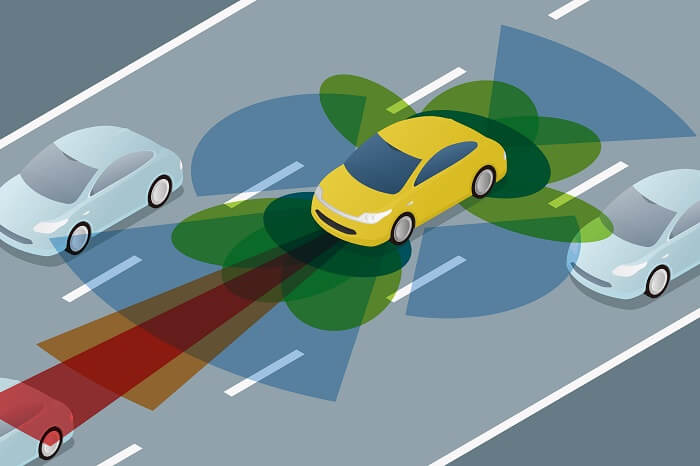
\includegraphics[width=0.41\textwidth]{Name_JFBR/car_sensors.jpg}}
 \caption {Fusionstyp: Kombinierte Fusion am Auto \cite{Ref_AutonousDrivingCriticism}}
 \label{Abb_AutoSensorenKombinierteFusion} 
\end{figure}
%+++++++++++++++++++++++++++++++++++++++++++++++++++++++++++++

%%%%%%%%%%%%%%%%%%%%%%%%%%%%%%%%%%%%%%%%%%%%%%%%%%%%%%%%%%%%%%%%%%%%%%%%%%%%%%%

\subsection*{Fusionsverfahren}

Die Fusion erfolgt nach einem bestimmten Verfahren. Das Verfahren ist abh�ngig von der Ebene, auf der die Fusion stattfinden soll. Im Folgenden werden die einzelnen Verfahren erl�utert.

\subsubsection*{Fusion �ber Sensoren}

Die Fusion �ber Sensoren hinweg ist das Zusammenf�hren der Signale der einzelnen Sensoren, die das Gleiche messen \cite{Ref_KochMSDF}. Ein Beispiel hierf�r ist das Messen der Temperatur \cite{Ref_KochMSDF}. Das Zusammenf�hren der Messsignale findet somit noch vor den eigentlichen Schritten der Signalverarbeitung statt \cite{Ref_KochMSDF}.

\subsubsection*{Fusion �ber Eigenschaften}

Bei der Fusion �ber Eigenschaften werden einzelne Eigenschaften, die durch Sensoren erfasst wurden, wie beispielsweise die Temperatur, der Druck und die Feuchtigkeit zusammengef�hrt, um aus den einzelnen Eigenschaften eine neue Eigenschaft zu ermitteln, wie beispielsweise in diesem Fall den Luftbrechungsindex zu ermitteln \cite{Ref_KochMSDF}.

\subsubsection*{Fusion �ber Bereiche}

Bei der Fusion �ber Bereiche erfassen mehrere Sensoren die gleiche Eigenschaft, aber in unterschiedlichen r�umlichen Bereichen \cite{Ref_KochMSDF}. Die Daten der Sensoren werden zu einem Abbild fusioniert. Durch diese Fusion wird der Gesamtbereich der erfassten Eigenschaft vergr��ert \cite{Ref_KochMSDF}.

\subsubsection*{Fusion �ber Zeit}

Bei der Fusion �ber die Zeit werden �ltere Daten mit den aktuellen Daten kombiniert \cite{Ref_KochMSDF}. �ltere Daten k�nnen �ltere Messdaten oder auch Daten von der Kalibrierung sein \cite{Ref_KochMSDF}.

%%%%%%%%%%%%%%%%%%%%%%%%%%%%%%%%%%%%%%%%%%%%%%%%%%%%%%%%%%%%%%%%%%%%%%%%%%%%%%%

%\newpage
\section*{Vorteile}

Als erstes wird der Nachteil ausgeglichen, dass normalerweise nur ein Sensor verwendet wird. Bei der Sensordatenfusion werden mehrere Sensoren eingesetzt. Dies hat den Vorteil, dass die Sch�tzgenauigkeit verbessert wird \cite{Ref_StuekerHomogeneSDF}. Des Weiteren wird der Gesamterfassungsbereich durch den Einsatz von mehreren Sensoren vergr��ert \cite{Ref_StuekerHomogeneSDF}. 
Dar�ber hinaus wird auch eine Verbesserung der Ausfallsicherheit erreicht \cite{Ref_StuekerHomogeneSDF}. Dadurch d�rfen einzelne Sensoren auch ausfallen \cite{Ref_StuekerHomogeneSDF}, ohne dass sie die Funktionsf�higkeit einschr�nken. Aber durch den Ausfall von Sensoren bei der Sensordatenfusion kann sich die durch die Sensordatenfusion verbesserte Sch�tzgenauigkeit und Robustheit wieder verschlechtern \cite{Ref_UniSiegenSensor}. Auch die gewonnene Robustheit des Gesamtsystems kann sich durch den Ausfall mehrere Sensoren verschlechtern, da unter Umst�nden Sensoren ausfallen, die unter bestimmten Umweltbedingungen besser arbeiten, als andere. Um die Ausfallsicherheit nicht zu gef�hrden, werden die Sensoren mit Redundanz ausgelegt \cite{Ref_StuekerHomogeneSDF}. Es bedeutet, dass Sensoren, die zwingend erforderlich f�r die Sicherheit oder die Funktionsf�higkeit sind, mehrfach im Sensornetzwerk eingebunden werden.

Durch den Einsatz von mehreren Sensoren, die unterschiedliche Wahrnehmungsverfahren verwenden, beispielsweise Radar und Laserabstandssensoren, k�nnen die unterschiedlichen St�rken der Wahrnehmungsverfahren zusammengef�hrt werden und verbessern die Wahrnehmung des Erfassungsbereichs. Die Nachteile einzelner Wahrnehmungsverfahren der Sensoren, die unter bestimmten Umweltbedingungen entstehen k�nnen, werden ausgeglichen, da die Wahrnehmung in solchen F�llen beispielsweise haupts�chlich durch einen oder mehrere andere Sensoren �bernommen wird \cite{Ref_SDFquadrocopter}. Die F�higkeit die Umgebung ausreichend zu erfassen, wird somit auch in f�r einzelne Sensoren schwierigen Situationen gew�hrleistet.

Durch die Verwendung mehrerer Sensoren, die nach unterschiedlichen Wahrnehmungsverfahren arbeiten, k�nnen mehr Informationen der Umgebung erfasst werden \cite{Ref_UniSiegenSensor}.

Die Sensordatenfusion hat ebenfalls den Vorteil, dass g�nstigere Sensoren verwendet werden k�nnen. Ohne die Sensordatenfusion m�ssen Sensoren verwendet werden, dessen Einschr�nkungen nicht problematisch f�r den eingesetzten Zweck sind. In diesen F�llen sind die Sensoren, die dann aber ben�tigt werden sehr teuer. Wenn mehrere einzelne Sensoren verwendet werden, k�nnen die Sensoren unter Ber�cksichtigung des physikalischen Prinzips zur Wahrnehmung so gew�hlt werden, dass Einschr�nkungen einzelner Sensoren durch andere Sensoren im System ausgeglichen werden k�nnen \cite{Ref_SDFquadrocopter}.

%%%%%%%%%%%%%%%%%%%%%%%%%%%%%%%%%%%%%%%%%%%%%%%%%%%%%%%%%%%%%%%%%%%%%%%%%%%%%%%

%\newpage
\section*{Nachteile}

Umso mehr Sensoren verwendet werden sollen, desto schwieriger wird die Integration der Sensoren \cite{Ref_WikiSDF}. Gr�nde hierf�r sind der erh�hte Aufwand f�r die Verkabelung, der weitere notwendige Platz f�r die Sensoren, sowie die Versorgung der Sensoren mit Strom. Aus dem erh�hten Aufwand f�r die Verkabelung resultieren direkt steigende Kosten f�r die Verkabelung, um alle verbauten Sensoren einzubinden \cite{Ref_WikiSDF}.

Mit der Anzahl der Sensoren steigen ebenfalls die Datenmengen der Sensoren, die �ber die Kommunikationssysteme �bertragen werden. In einigen Situationen wird versucht die Datentransferraten im Kommunikationssystem zu erh�hen \cite{Ref_WikiSDF}, damit die gr��ere Datenmenge nicht f�r eine erhebliche Erh�hung der ben�tigten Zeit zur �bertragung der Daten an das Verarbeitungssystem.

K�nnen die Datentransferraten nicht so stark erh�ht werden, sodass der Mehraufwand f�r den Transfer der zus�tzlichen Datenmengen ausgeglichen werden kann, entsteht ein deutlich erh�hter Zeitbedarf f�r die �bertragung der Daten der Sensoren zum Verarbeitungsziel \cite{Ref_WikiSDF}.

Umso mehr Daten entstehen und genutzt werden sollen, desto gr��er wird der Verarbeitungsaufwand. Der gr��ere Verarbeitungsaufwand macht sich bemerkbar durch eine erh�hte Auslastung der Verarbeitungssysteme. Die erh�hte Auslastung kann dann, wenn nicht gen�gend Rechenleistung verf�gbar ist, zu erheblich erh�hten Zeitverz�gerungen f�hren.

Da nicht alle Sensoren die Umgebung zum gleichen Zeitpunkt erfassen und sich auch die Abtastzeiten gegebenenfalls unterscheiden, muss das Verarbeitungssystem einen erheblichen zus�tzlichen Aufwand betreiben, um die Daten der einzelnen unterschiedlichen Sensoren zu synchronisieren \cite{Ref_WikiSDF}.

%%%%%%%%%%%%%%%%%%%%%%%%%%%%%%%%%%%%%%%%%%%%%%%%%%%%%%%%%%%%%%%%%%%%%%%%%%%%%%%

\newpage
\section*{Einsatzgebiete}

Die Sensordatenfusion wird in vielen Bereichen eingesetzt. Vor allem in den Bereichen des autonomen Fahrens und des autonomen Fliegens hat es eine hohe Bedeutung. In diesen beiden Bereichen werden hohe und auch sicherheitskritische Anforderungen an die maschinelle Erfassung der Umgebung gestellt. Die Anforderungen gestatten die Verwendung eines einzelnen Sensors nicht mehr.

%%%%%%%%%%%%%%%%%%%%%%%%%%%%%%%%%%%%%%%%%%%%%%%%%%%%%%%%%%%%%%%%%%%%%%%%%%%%%%%
%\newpage

%------------------------------------------------------------------------------------------------------------------------
\section*{Zusammenfassung}

Cras sagittis, ligula quis condimentum laoreet, lacus nisl pretium ligula, sed rutrum ipsum erat in dui. Nam hendrerit velit in dui laoreet, sed eleifend libero commodo. Vivamus pharetra lacus ac viverra hendrerit. Pellentesque dignissim tempus tempor. Nullam sit amet justo libero.

%%%%%%%%%%%%%%%%%%%%%%%%%%%%%%%%%%%%%%%%%%%%%%%%%%%%%%%%%%%%%%%%%%%%%%%%%%%%%%%

\begin{thebibliography}{}

\bibitem{Ref_WikiSDF}
Wikipedia, Online Nachschlagewerk: \textit{"'Sensordatenfusion"'},\\  \href{https://de.wikipedia.org/wiki/Sensordatenfusion}{https://de.wikipedia.org/wiki/Sensordatenfusion}, April 2019

\bibitem{Ref_StuekerHomogeneSDF}
St�ker, Dirk: \textit{"'Heterogene Sensordatenfusion zur robusten Objektverfolgung im automobilen Stra�enverkehr"'},\\  \href{https://d-nb.info/972494464/34}{https://d-nb.info/972494464/34}, April 2019

\bibitem{Ref_AutonousDrivingCriticism}
Ptock, Julia: \textit{"'Autonomes Fahren: Verbraucherschutz kritisiert Gesetzesentwurf der Regierung"'},\\  \href{https://www.logistik-watchblog.de/neuheiten/844-autonomes-fahren-verbraucherschutz-kritisiert-gesetzesentwurf.html}{https://www.logistik-watchblog.de/neuheiten/844-autonomes-fahren-verbraucherschutz-kritisiert-gesetzesentwurf.html}, April 2019

\bibitem{Ref_KochMSDF}
Mitchell, Harvey B.: \textit{"'Multi-Sensor Data Fusion: An Introduction"'},\\  \href{https://d-nb.info/972494464/34}{https://d-nb.info/972494464/34}, 1. Auflage, Springer Berlin Heidelberg, 2007

\bibitem{Ref_UniSiegenSensor}
Universit�t-GH Siegen, Zentrum f�r Sensorsysteme: \textit{"'Sensordatenfusion mit Kalman-Filtern Optimale Informationsverarbeitung"'},\\  \href{https://www.uni-siegen.de/zess/profil/929604.pdf}{https://www.uni-siegen.de/zess/profil/929604.pdf}, April 2019

\bibitem{Ref_SDFquadrocopter}
Lange, Sven: \textit{"'Faktorgraph-basierte Sensordatenfusion zur Anwendung auf einem Quadrocopter"'},\\  \href{http://www.qucosa.de/fileadmin/data/qucosa/documents/13057/diss\_lasve\_final.pdf}{http://www.qucosa.de/fileadmin/data/qucosa/documents /13057/diss\_lasve\_final.pdf}, April 2019


\end{thebibliography}



\end{document}
%-----------------------------------------------------------------------------------------------------------------------
